\documentclass[aspectratio=169,12pt,t]{beamer}

% --- Theme: Metropolis (modern, clean) ---
\usetheme[progressbar=frametitle,numbering=fraction,block=fill]{metropolis}

% --- Fira Sans font (install texlive-fonts-extra if missing) ---
\IfFileExists{FiraSans.sty}{\usepackage[sfdefault]{FiraSans}}{}

% --- Light background with warm accent ---
\definecolor{mDarkTeal}{RGB}{35,55,59}
\definecolor{mLightBrown}{RGB}{235,228,216}
\definecolor{mAccent}{RGB}{140,70,20}

\setbeamercolor{normal text}{fg=mDarkTeal,bg=white}
\setbeamercolor{alerted text}{fg=mAccent}
\setbeamercolor{frametitle}{bg=mDarkTeal,fg=white}
\setbeamercolor{progress bar}{fg=mAccent,bg=mLightBrown}
\setbeamercolor{title separator}{fg=mAccent}
\setbeamercolor{progress bar in head/foot}{fg=mAccent,bg=mLightBrown}
\setbeamercolor{progress bar in section page}{fg=mAccent,bg=mLightBrown}

% --- Packages ---
\usepackage[utf8]{inputenc}
\usepackage{amsmath,amssymb,amsthm}
\usepackage{mathrsfs}
\usepackage{tikz}
\usetikzlibrary{arrows.meta,positioning,calc,decorations.pathreplacing,shapes,patterns}
\usepackage{pgfplots}
\pgfplotsset{compat=1.18}

% --- Semi-transparent white highlight for text on top of background images ---
\usepackage[most]{tcolorbox}

% Inline highlight: \hl{short text}
\newtcbox{\hl}{%
  nobeforeafter, tcbox raise base,
  colback=white, opacityback=0.6,
  colframe=white, opacityframe=0,
  sharp corners, boxsep=2pt, left=3pt, right=3pt, top=2pt, bottom=2pt%
}

% Block highlight: \begin{hlbox} ... \end{hlbox}  (multi-line, paragraphs, itemize)
% Optional argument accepts any tcolorbox key, e.g. [width=0.6\linewidth]
\newtcolorbox{hlbox}[1][]{%
  enhanced, breakable,
  colback=white, opacityback=0.6,
  colframe=white, opacityframe=0,
  boxsep=3pt, left=6pt, right=6pt, top=4pt, bottom=4pt,
  sharp corners,
  {#1}%
}

% --- Custom colors for content types ---
\definecolor{defcolor}{RGB}{25,85,120}
\definecolor{thmcolor}{RGB}{140,35,35}
\definecolor{proofcolor}{RGB}{35,100,50}
\definecolor{excolor}{RGB}{140,75,10}
\definecolor{remcolor}{RGB}{90,90,90}

% --- Beamer blocks for mathematical content types (semi-transparent) ---
\tcbset{hlblockbase/.style={
  enhanced, breakable,
  coltitle=white, fonttitle=\bfseries,
  opacitybacktitle=0.8, opacityback=0.6,
  opacityframe=0,
  sharp corners,
  boxsep=1pt, left=5pt, right=5pt, top=2pt, bottom=2pt,
  toptitle=1pt, bottomtitle=1pt
}}

\newtcolorbox{defblock}[1]{hlblockbase, title={#1},
  colbacktitle=defcolor, colback=defcolor!15, colframe=defcolor}
\newtcolorbox{thmblock}[1]{hlblockbase, title={#1},
  colbacktitle=thmcolor, colback=thmcolor!15, colframe=thmcolor}
\newtcolorbox{proofblock}[1]{hlblockbase, title={#1},
  colbacktitle=proofcolor, colback=proofcolor!15, colframe=proofcolor}
\newtcolorbox{exblock}[1]{hlblockbase, title={#1},
  colbacktitle=excolor, colback=excolor!15, colframe=excolor}
\newtcolorbox{remblock}[1]{hlblockbase, title={#1},
  colbacktitle=remcolor, colback=remcolor!15, colframe=remcolor}

% --- Metadata ---
\title{Chapter 3: Numerical Sequences and Series}
\subtitle{Section: Subsequences}
\author{Based on Walter Rudin's \emph{Principles of Mathematical Analysis}}
\date{}

\begin{document}

% =============================================================================
% TITLE AND OUTLINE
% =============================================================================
{
\usebackgroundtemplate{%
  
\includegraphics[width=\paperwidth,height=\paperheight,keepaspectratio=false]{chapter_03_bg_00.png}%
}
\begin{frame}[plain]
  \titlepage
  \note{
    Welcome back to Chapter 3 of Principles of Mathematical Analysis. In
    the previous section we introduced convergent sequences in a metric
    space. In this short but important section we widen the lens: even
    when a sequence as a whole fails to converge, it may contain pieces
    that do. Those pieces are called subsequences, and they will become
    one of the most useful tools in the book. We will define
    subsequences, prove that compact spaces always force a convergent
    subsequence to exist, and show that the set of all subsequential
    limits of any sequence is a closed set.
  }
\end{frame}
}

{
\usebackgroundtemplate{%
  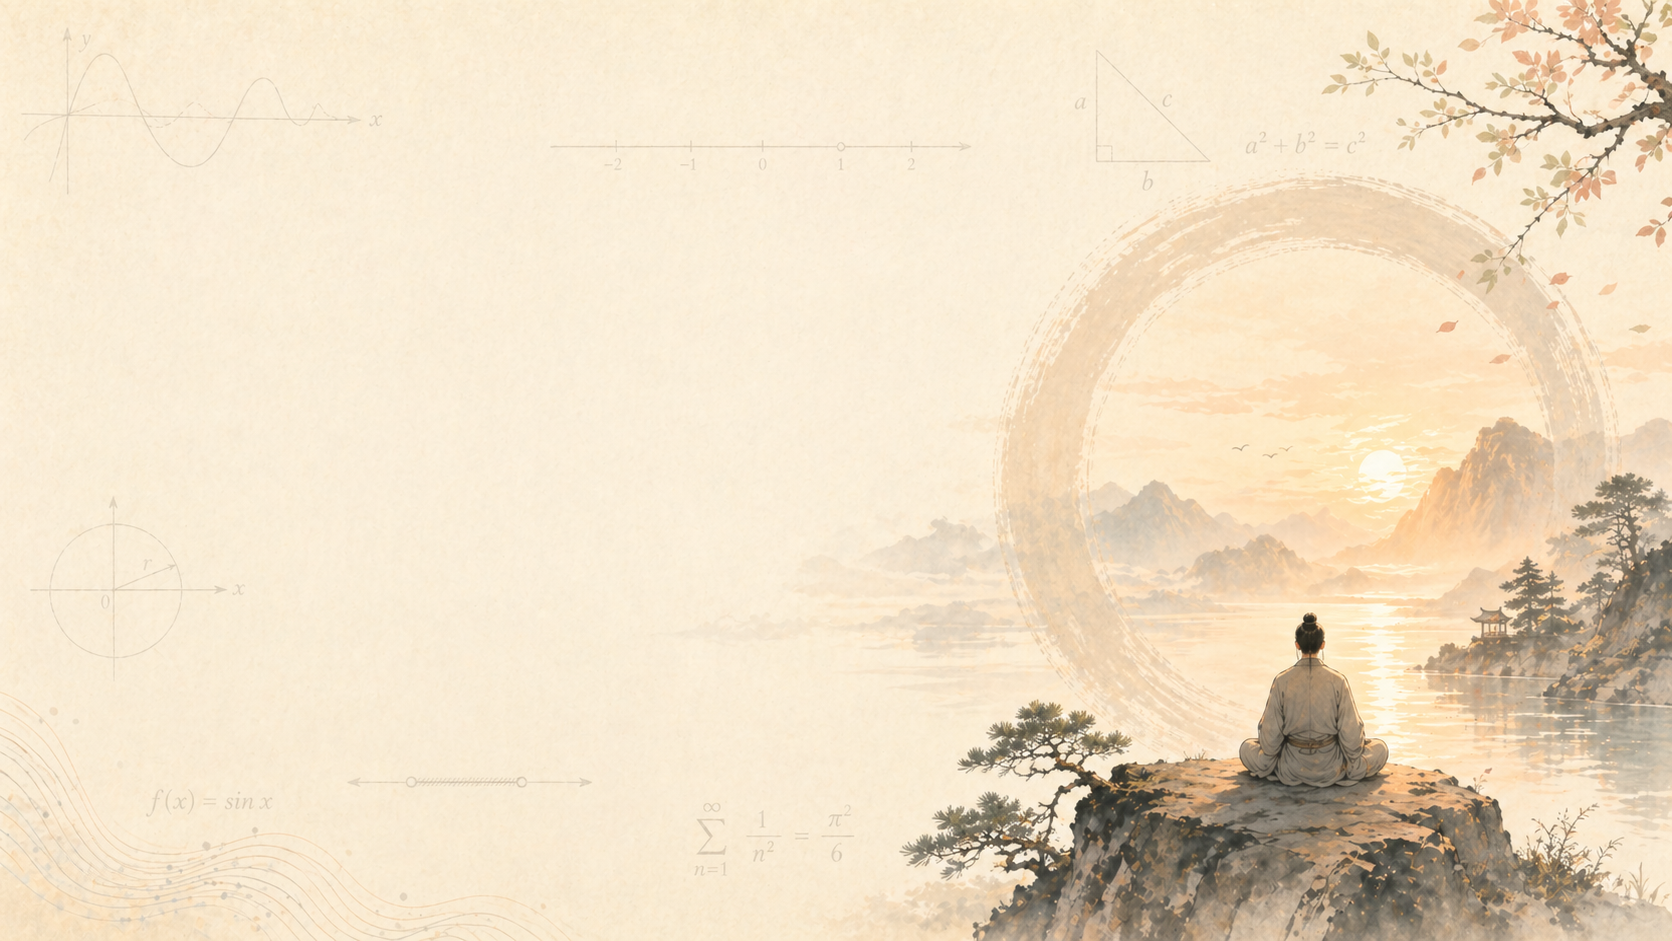
\includegraphics[width=\paperwidth,height=\paperheight,keepaspectratio=false]{chapter_03_bg_01.png}%
}
\begin{frame}[c]{Outline}
  \begin{center}
    \tableofcontents
  \end{center}
  \note{
    Here is the plan. We start with motivation, asking why subsequences
    are worth our attention. Then we give Definition 3.5, which makes
    the notion of a subsequence precise, and we record the basic remark
    that a sequence converges to "p" if and only if every subsequence
    does. Next comes Theorem 3.6, the existence theorem, which says that
    every sequence in a compact metric space, and every bounded sequence
    in "R" to the "k", has a convergent subsequence. We work through the
    proof in detail. Then comes Theorem 3.7, which says the set of
    subsequential limits is always a closed subset of the metric space,
    and again we work through the proof. We close with a summary.
  }
\end{frame}

% =============================================================================
% MOTIVATION
% =============================================================================
\section{Motivation}

% --- Build 1/3 ---
\begin{frame}{Why Subsequences?}
  \begin{hlbox}
    \begin{itemize}
      \item Many sequences \alert{do not converge} \dots\ but still have structure
    \end{itemize}
  \end{hlbox}

  \note{
    Many sequences we encounter in analysis simply do not converge. The
    sequence of plus and minus ones, for instance, oscillates forever.
    The sequence whose "n"-th term is "n" runs off to infinity. These
    sequences have no limit, but it would be wasteful to just throw them
    away. They still carry plenty of internal structure, and the right
    way to see it is to look at parts of the sequence rather than the
    sequence as a whole.
  }
\end{frame}

% --- Build 2/3 ---
\begin{frame}{Why Subsequences?}
  \begin{hlbox}
    \begin{itemize}
      \item Many sequences \alert{do not converge} \dots\ but still have structure
      \item A \alert{subsequence} extracts a thinned-out piece that may converge
    \end{itemize}
  \end{hlbox}

  \note{
    A subsequence is what you get by keeping infinitely many terms of
    the original sequence in their original order, while discarding the
    rest. Even when the full sequence has no limit, a clever choice of
    subsequence may pick out a single accumulation point and converge to
    it. For the alternating plus-minus-one sequence, taking only the
    even-indexed terms gives a subsequence that converges to plus one,
    and the odd-indexed terms give one that converges to minus one.
  }
\end{frame}

% --- Build 3/3 ---
\begin{frame}{Why Subsequences?}
  \begin{hlbox}
    \begin{itemize}
      \item Many sequences \alert{do not converge} \dots\ but still have structure
      \item A \alert{subsequence} extracts a thinned-out piece that may converge
      \item In \alert{compact} spaces, a convergent subsequence \emph{always exists}
    \end{itemize}
  \end{hlbox}

  \note{
    The big payoff comes in compact metric spaces. There, no matter how
    badly the original sequence oscillates, we are guaranteed to be
    able to extract a subsequence that converges to some point of the
    space. This is the Bolzano-Weierstrass principle in disguise, and
    it is the core existence result of the section. With it in hand we
    can prove that limits exist without having to construct them
    explicitly. Let us start with the definition.
  }
\end{frame}
}

{
\usebackgroundtemplate{%
  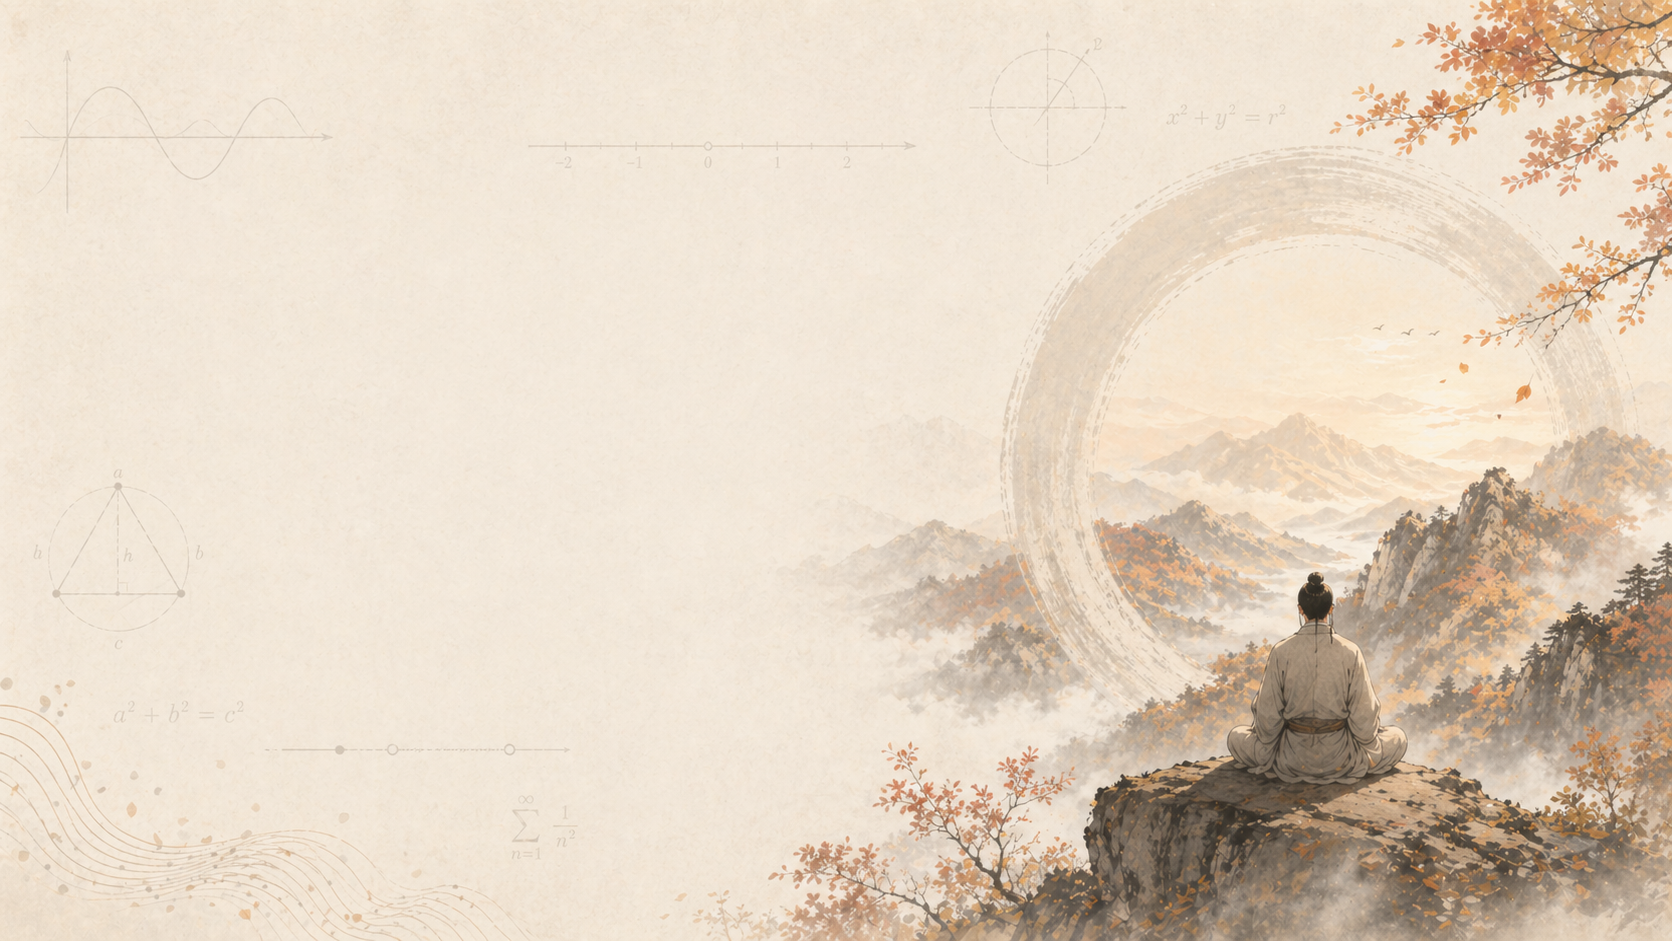
\includegraphics[width=\paperwidth,height=\paperheight,keepaspectratio=false]{chapter_03_bg_02.png}%
}
% =============================================================================
% DEFINITION 3.5
% =============================================================================
\section{Definition of a Subsequence}

% --- Def 3.5: Build 1/2 ---
\begin{frame}{Definition 3.5: Subsequence}
  \begin{defblock}{Definition 3.5 --- Subsequence}
    Given a sequence $\{p_n\}$ and a sequence of \alert{positive integers}
    \[
      n_1 < n_2 < n_3 < \cdots ,
    \]
    the sequence $\{p_{n_k}\}$ is called a \alert{subsequence} of $\{p_n\}$.
  \end{defblock}

  \note{
    Here is the formal definition. We begin with a sequence "p" sub
    "n". Choose any infinite, strictly increasing list of positive
    integers, call them "n" sub 1, "n" sub 2, "n" sub 3, and so on.
    Now read the original sequence at those chosen indices: the result
    is a new sequence, which we call a subsequence and write as "p"
    sub "n" sub "k". Two features matter. First, the indices must be
    strictly increasing, which means we keep the original order and
    never revisit. Second, there must be infinitely many of them, so
    that what we get is itself a sequence rather than a finite list.
    A useful mental picture: the subsequence is the original with
    some terms erased, but the surviving terms left in their original
    order.
  }
\end{frame}

% --- Def 3.5: Build 2/2 ---
\begin{frame}{Definition 3.5: Subsequential Limit}
  \begin{defblock}{Definition 3.5 --- Subsequential Limit}
    Given $\{p_n\}$ and a subsequence $\{p_{n_k}\}$:
    \begin{itemize}
      \item If $\{p_{n_k}\}$ converges, its limit is a \alert{subsequential limit} of $\{p_n\}$.
      \item Write $E^*$ for the set of all subsequential limits.
    \end{itemize}
  \end{defblock}

  \note{
    Now suppose a particular subsequence happens to converge. Its limit
    is then called a subsequential limit of the original sequence. The
    original sequence may have many subsequential limits, just one, or
    none at all. Throughout this section we will denote the set of all
    subsequential limits by "E" star. We will see in a few slides that
    "E" star is always a closed subset of the ambient metric space, no
    matter what the sequence looks like.
  }
\end{frame}

% --- Picture: subsequence as thinning ---
\begin{frame}{Picture: A Subsequence Is a Thinned Sequence}
  \begin{center}
  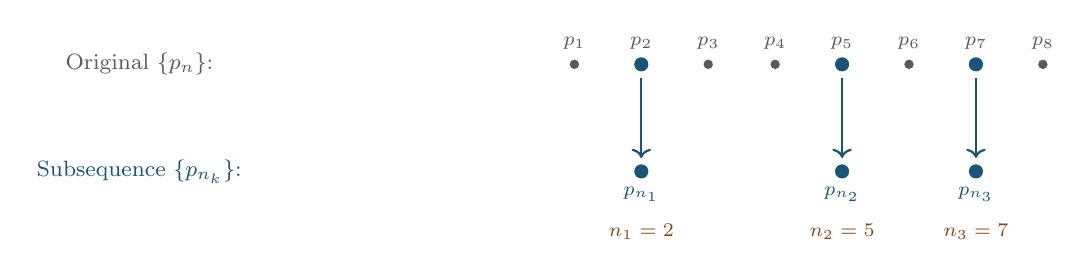
\begin{tikzpicture}[scale=0.85]
    % Original sequence row
    \node[remcolor] at (-5.5, 1.6) {\footnotesize Original $\{p_n\}$:};
    \foreach \x/\lab in {1/p_1, 2/p_2, 3/p_3, 4/p_4, 5/p_5, 6/p_6, 7/p_7, 8/p_8} {
      \fill[remcolor] (\x, 1.6) circle (2pt);
      \node[remcolor, above=2pt] at (\x, 1.6) {\scriptsize $\lab$};
    }
    % Selected indices: 2, 5, 7
    \fill[defcolor] (2, 1.6) circle (3pt);
    \fill[defcolor] (5, 1.6) circle (3pt);
    \fill[defcolor] (7, 1.6) circle (3pt);
    % Arrows down to subsequence row
    \draw[defcolor, ->, thick] (2, 1.4) -- (2, 0.2);
    \draw[defcolor, ->, thick] (5, 1.4) -- (5, 0.2);
    \draw[defcolor, ->, thick] (7, 1.4) -- (7, 0.2);
    % Subsequence row
    \node[defcolor] at (-5.5, 0) {\footnotesize Subsequence $\{p_{n_k}\}$:};
    \fill[defcolor] (2, 0) circle (3pt);
    \node[defcolor, below=2pt] at (2, 0) {\scriptsize $p_{n_1}$};
    \fill[defcolor] (5, 0) circle (3pt);
    \node[defcolor, below=2pt] at (5, 0) {\scriptsize $p_{n_2}$};
    \fill[defcolor] (7, 0) circle (3pt);
    \node[defcolor, below=2pt] at (7, 0) {\scriptsize $p_{n_3}$};
    % Index labels
    \node[mAccent] at (2, -0.9) {\scriptsize $n_1 = 2$};
    \node[mAccent] at (5, -0.9) {\scriptsize $n_2 = 5$};
    \node[mAccent] at (7, -0.9) {\scriptsize $n_3 = 7$};
  \end{tikzpicture}
  \end{center}

  \vspace{0.3em}
  \begin{center}
    \hl{\emph{Keep some terms (in order), drop the rest.}}
  \end{center}

  \note{
    Here is the visual idea. The top row shows the original sequence.
    The gray dots are all the terms, indexed 1 through 8 in this picture.
    To form a subsequence, we choose a strictly increasing list of
    indices, here 2, 5, and 7, highlighted in blue. Reading off the
    sequence at those indices gives us a new shorter sequence, shown on
    the bottom row, whose first term is the original term at index 2,
    second term is the original at index 5, and third term is the
    original at index 7. The original order is preserved; we never go
    back. In the actual definition we keep going forever, picking
    infinitely many indices, but the picture shows the basic operation.
  }
\end{frame}

% --- Example: alternating sequence ---
\begin{frame}{Example: $p_n = (-1)^n$}
  \begin{exblock}{Two Subsequential Limits}
    Let $p_n = (-1)^n$ in $\mathbb{R}$. The sequence $\{p_n\}$ \alert{diverges}, but:
    \vspace{0.2em}
    \begin{itemize}
      \item Even indices ($n_k = 2k$): \;\; $p_{n_k} = 1 \to 1$.
      \item Odd indices ($n_k = 2k-1$): \;\; $p_{n_k} = -1 \to -1$.
    \end{itemize}
    \vspace{0.2em}
    So $E^* = \{-1, +1\}$.
  \end{exblock}

  \note{
    Here is the simplest illustrative example. Take the sequence
    whose "n"-th term is minus one to the "n", in the real line. So
    the sequence reads minus one, plus one, minus one, plus one, and
    so on forever. As a whole this sequence does not converge. But if
    we keep only the even-indexed terms we get the constant sequence
    plus one, which trivially converges to plus one. If we keep only
    the odd-indexed terms we get the constant sequence minus one,
    which converges to minus one. So the set "E" star here has two
    elements, plus one and minus one. This is our first concrete
    look at "E" star: it can be richer than just the empty set or a
    single limit, and the point of Theorem 3.7 a few slides from now
    will be to pin down the one structural property "E" star always
    has, regardless of how strange the original sequence is.
  }
\end{frame}

% --- Remark: convergence iff every subsequence converges ---
\begin{frame}{Remark: Convergence and Subsequences}
  \begin{remblock}{Useful Equivalence}
    \[
      p_n \to p
      \quad \iff \quad
      \text{every subsequence } \{p_{n_k}\} \text{ converges to } p.
    \]
  \end{remblock}

  \vspace{0.4em}
  \begin{hlbox}
    \textbf{Two-way picture:}
    \begin{itemize}
      \item ($\Rightarrow$) Tail of $\{p_n\}$ in $\varepsilon$-ball $\Longrightarrow$ tail of $\{p_{n_k}\}$ in $\varepsilon$-ball.
      \item ($\Leftarrow$) The original $\{p_n\}$ \emph{is itself} a subsequence.
    \end{itemize}
  \end{hlbox}

  \note{
    Rudin records, without writing out a formal proof, a useful
    equivalence: a sequence "p" sub "n" converges to "p" if and only if
    every subsequence of "p" sub "n" also converges to "p". Both
    directions are easy to see. Going forward, suppose the full sequence
    converges to "p". Pick any epsilon greater than zero. From some
    index "N" on, every term of the original sequence is within distance
    epsilon of "p". Now the indices "n" sub "k" form a strictly
    increasing sequence of positive integers, so "n" sub "k" is at
    least "k" for every "k". Hence once "k" is at least "N", "n" sub
    "k" is also at least "N", and the subsequence term is within
    epsilon of "p" as well. Going backward, the original sequence is
    itself a subsequence, the trivial one with indices 1, 2, 3, and so
    on, so if every subsequence converges to "p", in particular the
    original does.
  }
\end{frame}
}

{
\usebackgroundtemplate{%
  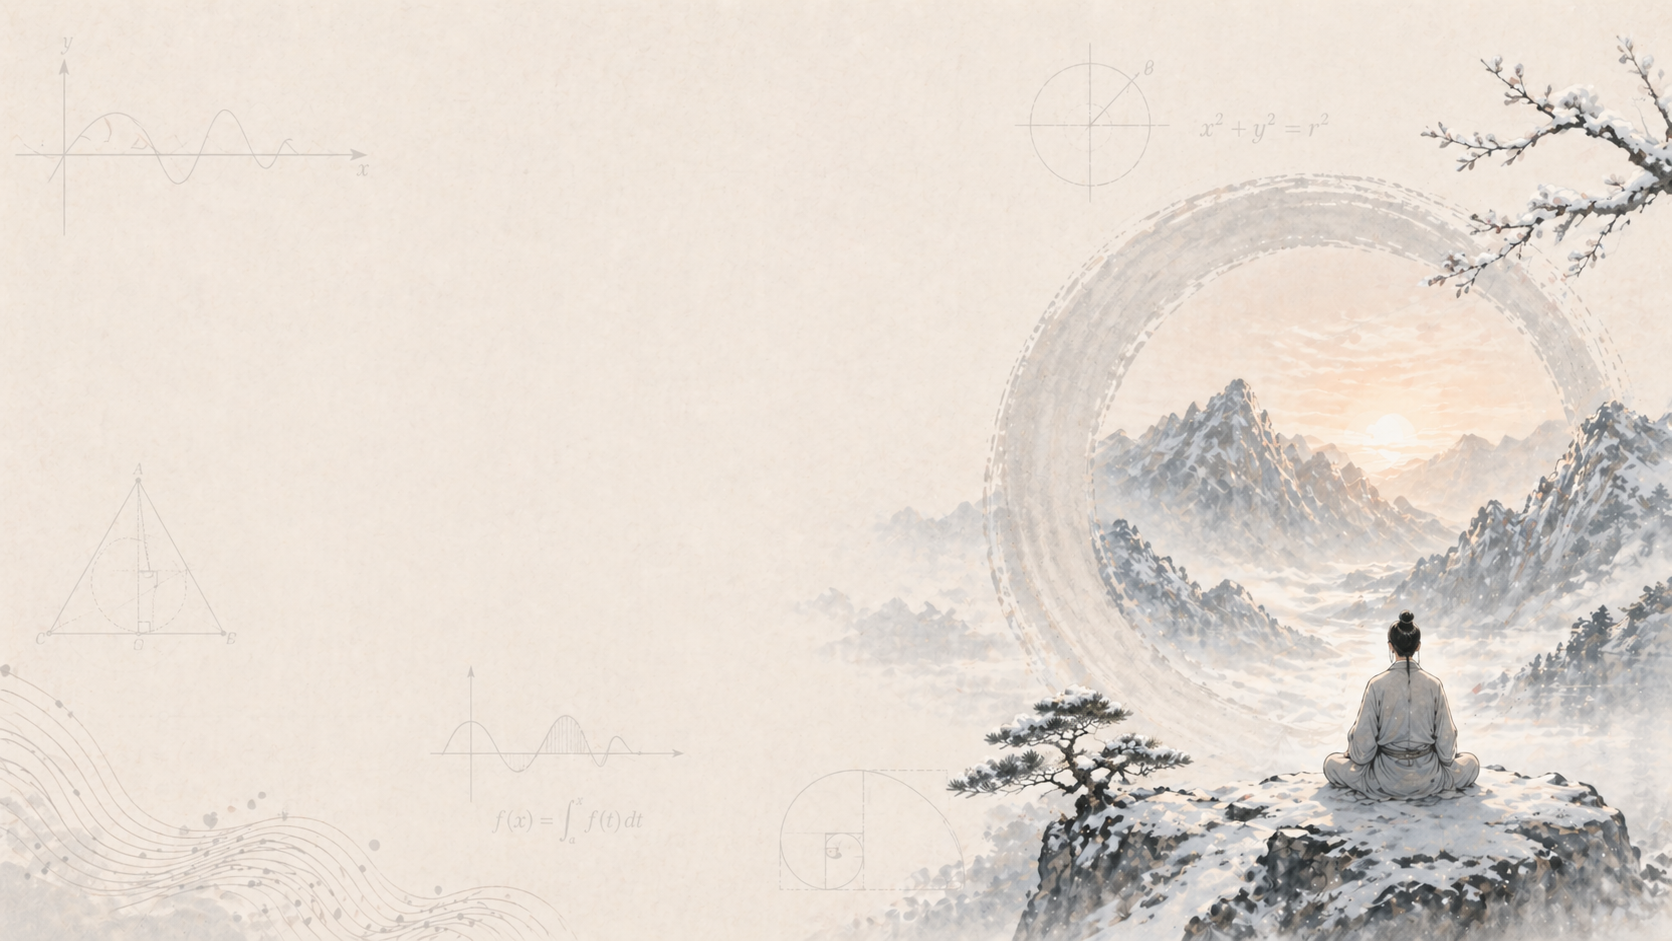
\includegraphics[width=\paperwidth,height=\paperheight,keepaspectratio=false]{chapter_03_bg_03.png}%
}
% =============================================================================
% THEOREM 3.6
% =============================================================================
\section{Existence of Convergent Subsequences}

% --- Theorem 3.6: Build 1/2 ---
\begin{frame}{Theorem 3.6: Compactness Forces Convergence}
  \begin{thmblock}{Theorem 3.6 (a)}
    If $\{p_n\}$ is a sequence in a \alert{compact} metric space $X$,
    then some subsequence of $\{p_n\}$ converges to a point of $X$.
  \end{thmblock}

  \note{
    Here is the main result of the section, in two parts. Part "a"
    states the abstract version: in any compact metric space, every
    sequence, no matter how wildly it behaves, has at least one
    subsequence that converges to some point of the space. Compactness
    is exactly the property that makes this work. We will give a
    detailed proof in a moment.
  }
\end{frame}

% --- Theorem 3.6: Build 2/2 ---
\begin{frame}{Theorem 3.6: Compactness Forces Convergence}
  \begin{thmblock}{Theorem 3.6 (a)}
    If $\{p_n\}$ is in a \alert{compact} metric space $X$, then some subsequence converges in $X$.
  \end{thmblock}

  \begin{thmblock}{Theorem 3.6 (b)}
    Every \alert{bounded} sequence in $\mathbb{R}^k$ contains a convergent subsequence.
  \end{thmblock}

  \note{
    Part "b" specialises to euclidean space. In "R" to the "k", every
    bounded sequence has a convergent subsequence. This is the
    classical Bolzano-Weierstrass theorem, which the reader may have
    seen before for the real line. Here it appears as a quick corollary
    of part "a", because by Theorem 2.41 every bounded subset of "R" to
    the "k" sits inside a compact set, and once we are in a compact set,
    part "a" applies.
  }
\end{frame}

% --- Proof strategy ---
\begin{frame}{Proof Strategy: Theorem 3.6 (a)}
  \begin{hlbox}
    \textbf{Goal:} Build a convergent subsequence of $\{p_n\}$ inside compact $X$.

    \vspace{0.6em}
    \textbf{Two cases by the range $E = \{p_n : n \geq 1\}$:}
    \begin{enumerate}
      \item[(I)] $E$ is \alert{finite}: some value $p$ is hit infinitely often $\Rightarrow$ constant subsequence.
      \item[(II)] $E$ is \alert{infinite}: by Theorem 2.37, $E$ has a limit point $p \in X$. \\
                 Build a subsequence inductively, using $\varepsilon = 1/k$ at step $k$.
    \end{enumerate}
  \end{hlbox}

  \note{
    Before we write out the proof, here is the high-level strategy. The
    range "E" of the sequence is the set of points that actually appear
    among the terms. Two cases: either "E" is a finite set, or "E" is
    an infinite set. In the finite case, pigeonhole gives us a single
    value that is hit infinitely many times, and the constant
    subsequence at that value converges trivially. In the infinite case
    we invoke Theorem 2.37, which states that every infinite subset of
    a compact set has a limit point in the set. Once we have such a
    limit point "p", we build a subsequence that hugs "p" by an
    inductive construction, demanding the "k"-th chosen term lie within
    distance one over "k" of "p".
  }
\end{frame}

% --- Proof of 3.6(a): finite case ---
\begin{frame}{Proof of 3.6 (a) --- Case I: $E$ Finite}
  \begin{proofblock}{Case I: finite range}
    If $E = \{p_n : n \geq 1\}$ is finite, some value $p \in E$ is taken \alert{infinitely often}:
    \[
      p_{n_1} = p_{n_2} = p_{n_3} = \cdots = p,
      \quad n_1 < n_2 < n_3 < \cdots .
    \]
    The constant subsequence $\{p_{n_k}\}$ converges to $p \in X$. \quad $\Box$
  \end{proofblock}

  \note{
    Here is the finite case in full. Suppose the range "E" of the
    sequence is finite. Since the sequence has infinitely many terms but
    only finitely many possible values, by the pigeonhole principle some
    single value, call it "p", is taken infinitely many times. List the
    indices at which "p" appears as "n" sub 1 less than "n" sub 2 less
    than "n" sub 3, and so on. The corresponding subsequence is the
    constant sequence "p", "p", "p", and so on, which obviously
    converges to "p". And "p" lies in "E", which is a subset of "X",
    so the limit is indeed in "X". The first case is done.
  }
\end{frame}

% --- Proof of 3.6(a): infinite case, Step 1 ---
\begin{frame}{Proof of 3.6 (a) --- Case II: Step 1}
  \begin{proofblock}{Case II: $E$ infinite, Step 1 --- find a limit point}
    By \alert{Theorem 2.37}, every infinite subset of a compact set has a limit point in the set.
    \[
      \Longrightarrow \quad E \text{ has a limit point } p \in X.
    \]
  \end{proofblock}

  \note{
    Now the infinite case. Recall Theorem 2.37 from Chapter 2, which
    says that every infinite subset of a compact metric space has a
    limit point inside that space. Apply it to "E", which is an
    infinite subset of the compact space "X". The conclusion is that
    "E" has at least one limit point "p", and "p" lies in "X". This
    "p" is going to be the limit of our subsequence; we now have to
    construct the subsequence.
  }
\end{frame}

% --- Proof of 3.6(a): infinite case, Step 2 ---
\begin{frame}{Proof of 3.6 (a) --- Case II: Step 2}
  \begin{proofblock}{Step 2 --- pick the first index $n_1$}
    Since $p$ is a limit point of $E$, every neighborhood of $p$ contains points of $E$ other than $p$.

    \vspace{0.3em}
    Choose $n_1$ with
    \[
      d(p, p_{n_1}) < 1.
    \]
  \end{proofblock}

  \note{
    Step 2: pick the first index. Because "p" is a limit point of "E",
    every neighborhood of "p", no matter how small, contains points of
    "E" different from "p". In particular, the open ball of radius one
    around "p" contains some term of the sequence. Let "n" sub 1 be any
    index whose term lies inside that ball. Then the distance from "p"
    to that term is less than one. This is the first step of the
    subsequence.
  }
\end{frame}

% --- Proof of 3.6(a): infinite case, Step 3 ---
\begin{frame}{Proof of 3.6 (a) --- Case II: Step 3}
  \begin{proofblock}{Step 3 --- inductive choice of $n_k$}
    Suppose $n_1 < n_2 < \cdots < n_{k-1}$ have been chosen.

    \vspace{0.3em}
    By \alert{Theorem 2.20}: every neighborhood of a limit point contains \emph{infinitely many} points of $E$.

    \vspace{0.3em}
    So there is $n_k > n_{k-1}$ with
    \[
      d(p, p_{n_k}) < \frac{1}{k}.
    \]
  \end{proofblock}

  \note{
    Step 3: the inductive step. Assume we have already chosen the first
    "k" minus one indices, in increasing order. We need to pick the
    next one. The key fact, recorded as Theorem 2.20 back in Chapter 2,
    is that every neighborhood of a limit point contains infinitely
    many points of "E". So the open ball of radius one over "k" around
    "p" contains infinitely many terms of the sequence. In particular,
    there are infinitely many indices "n" with that property, and we
    can pick one larger than "n" sub "k" minus one. Call it "n" sub
    "k". The distance from "p" to that term is then less than one over
    "k". By induction this process can continue forever.
  }
\end{frame}

% --- Picture: bounded -> compact -> subsequence ---
\begin{frame}{Picture: Inductive Construction of the Subsequence}
  \begin{center}
  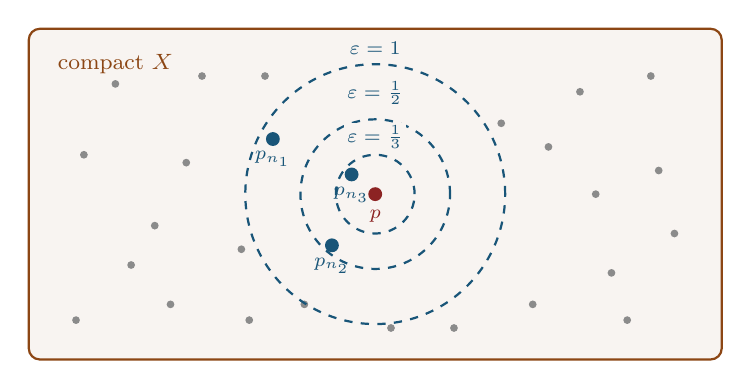
\begin{tikzpicture}[scale=1.0]
    % Compact ambient
    \fill[mAccent!6, rounded corners=4pt] (-4.4, -2.1) rectangle (4.4, 2.1);
    \draw[mAccent, thick, rounded corners=4pt] (-4.4, -2.1) rectangle (4.4, 2.1);
    \node[mAccent, above] at (-3.3, 1.4) {\footnotesize compact $X$};
    % Background sequence points scattered far from p (drawn first)
    \foreach \x/\y in {-3.8/-1.6, -3.3/1.4, -2.8/-0.4, -2.2/1.5, -1.6/-1.6, -2.4/0.4, 1.0/-1.7, 2.6/1.3, 3.0/-1.0, 3.6/0.3, 3.2/-1.6, -0.9/-1.4, 2.0/-1.4, -3.7/0.5, 2.8/0.0, -1.7/-0.7, 0.2/-1.7, -3.1/-0.9, -1.4/1.5, 3.5/1.5, 2.2/0.6, -2.6/-1.4, 1.6/0.9, 3.8/-0.5} {
      \fill[remcolor!70] (\x, \y) circle (1.4pt);
    }
    % Concentric epsilon-balls: radius 1, 1/2, 1/3
    \draw[defcolor, thick, dashed] (0,0) circle (1.65);
    \draw[defcolor, thick, dashed] (0,0) circle (0.95);
    \draw[defcolor, thick, dashed] (0,0) circle (0.5);
    % Radius labels stacked vertically above p (clear region)
    \node[defcolor, fill=mAccent!6, inner sep=1pt] at (0, 1.85) {\scriptsize $\varepsilon = 1$};
    \node[defcolor, fill=mAccent!6, inner sep=1pt] at (0, 1.28) {\scriptsize $\varepsilon = \tfrac{1}{2}$};
    \node[defcolor, fill=mAccent!6, inner sep=1pt] at (0, 0.72) {\scriptsize $\varepsilon = \tfrac{1}{3}$};
    % Limit point p
    \fill[thmcolor] (0, 0) circle (2.5pt);
    \node[thmcolor, below=1pt] at (0, -0.05) {\scriptsize $p$};
    % Selected subsequence terms (left/below half of figure)
    % p_{n_1}: inside r=1.65, outside r=0.95  (dist = 1.47)
    \fill[defcolor] (-1.30, 0.70) circle (2.5pt);
    \node[defcolor, below=1pt] at (-1.30, 0.70) {\scriptsize $p_{n_1}$};
    % p_{n_2}: inside r=0.95, outside r=0.5   (dist = 0.85)
    \fill[defcolor] (-0.55, -0.65) circle (2.5pt);
    \node[defcolor, below=1pt] at (-0.55, -0.65) {\scriptsize $p_{n_2}$};
    % p_{n_3}: inside r=0.5                   (dist = 0.39)
    \fill[defcolor] (-0.30, 0.25) circle (2.5pt);
    \node[defcolor, below=1pt] at (-0.30, 0.25) {\scriptsize $p_{n_3}$};
  \end{tikzpicture}
  \end{center}

  \vspace{0.2em}
  \begin{center}
    \hl{\emph{Each step shrinks $\varepsilon$ to $1/k$ and pulls one new term into the smaller ball.}}
  \end{center}

  \note{
    Here is the geometric picture of the inductive construction. The
    orange-shaded box represents the compact metric space "X". The
    central red dot is the limit point "p" supplied by Theorem 2.37.
    The three dashed blue circles around "p" have radii one, one half,
    and one third, the values of epsilon used at steps 1, 2, and 3 of
    the proof. The gray dots scattered around are terms of the original
    sequence. At each step we use the fact that "p" is a limit point of
    "E" to find a sequence term inside the corresponding ball. The
    three highlighted blue terms are the chosen subsequence: the first
    inside the unit ball, the second inside the one half ball, the
    third inside the one third ball. As the radius shrinks toward zero,
    the chosen terms march in toward "p".
  }
\end{frame}

% --- Proof of 3.6(a): infinite case, Step 4 ---
\begin{frame}{Proof of 3.6 (a) --- Case II: Step 4}
  \begin{proofblock}{Step 4 --- the subsequence converges to $p$}
    For all $k \geq 1$:
    \[
      d(p, p_{n_k}) < \frac{1}{k}.
    \]
    Given $\varepsilon > 0$, choose $N \geq 1/\varepsilon$. Then for all $k \geq N$:
    \[
      d(p, p_{n_k}) < \frac{1}{k} \leq \frac{1}{N} \leq \varepsilon.
    \]
    Hence $p_{n_k} \to p \in X$. \quad $\Box$
  \end{proofblock}

  \note{
    Step 4 closes the proof. By construction, for every "k" the "k"-th
    term of the chosen subsequence lies within distance one over "k" of
    "p". Now pick any tolerance epsilon greater than zero, and choose
    a positive integer "N" at least one over epsilon. For every "k" at
    least "N", the distance from "p" to the "k"-th subsequential term
    is less than one over "k", which is at most one over "N", which is
    at most epsilon. So the subsequence converges to "p", and "p" lies
    in "X". The proof of part "a" is complete.
  }
\end{frame}

% --- Proof of 3.6(b) ---
\begin{frame}{Proof of 3.6 (b) --- The Bounded Case in $\mathbb{R}^k$}
  \begin{proofblock}{Reduction to part (a)}
    Let $\{p_n\}$ be a bounded sequence in $\mathbb{R}^k$.
    \vspace{0.2em}
    \begin{itemize}
      \item \alert{Theorem 2.41}: every bounded subset of $\mathbb{R}^k$ lies in a compact set $K$.
      \item So $\{p_n\}$ is a sequence in compact $K$.
      \item Apply part (a) $\Longrightarrow$ a subsequence converges in $K \subset \mathbb{R}^k$. \;$\Box$
    \end{itemize}
  \end{proofblock}

  \note{
    Part "b" follows quickly. Let "p" sub "n" be a bounded sequence in
    "R" to the "k". By Theorem 2.41, every bounded subset of "R" to the
    "k" sits inside some compact set "K". So our bounded sequence is in
    fact a sequence in the compact set "K". Apply part "a" to get a
    subsequence that converges to a point of "K", which in particular
    is a point of "R" to the "k". This is the classical
    Bolzano-Weierstrass theorem for euclidean space, and it now follows
    almost for free from the abstract version.
  }
\end{frame}
}

{
\usebackgroundtemplate{%
  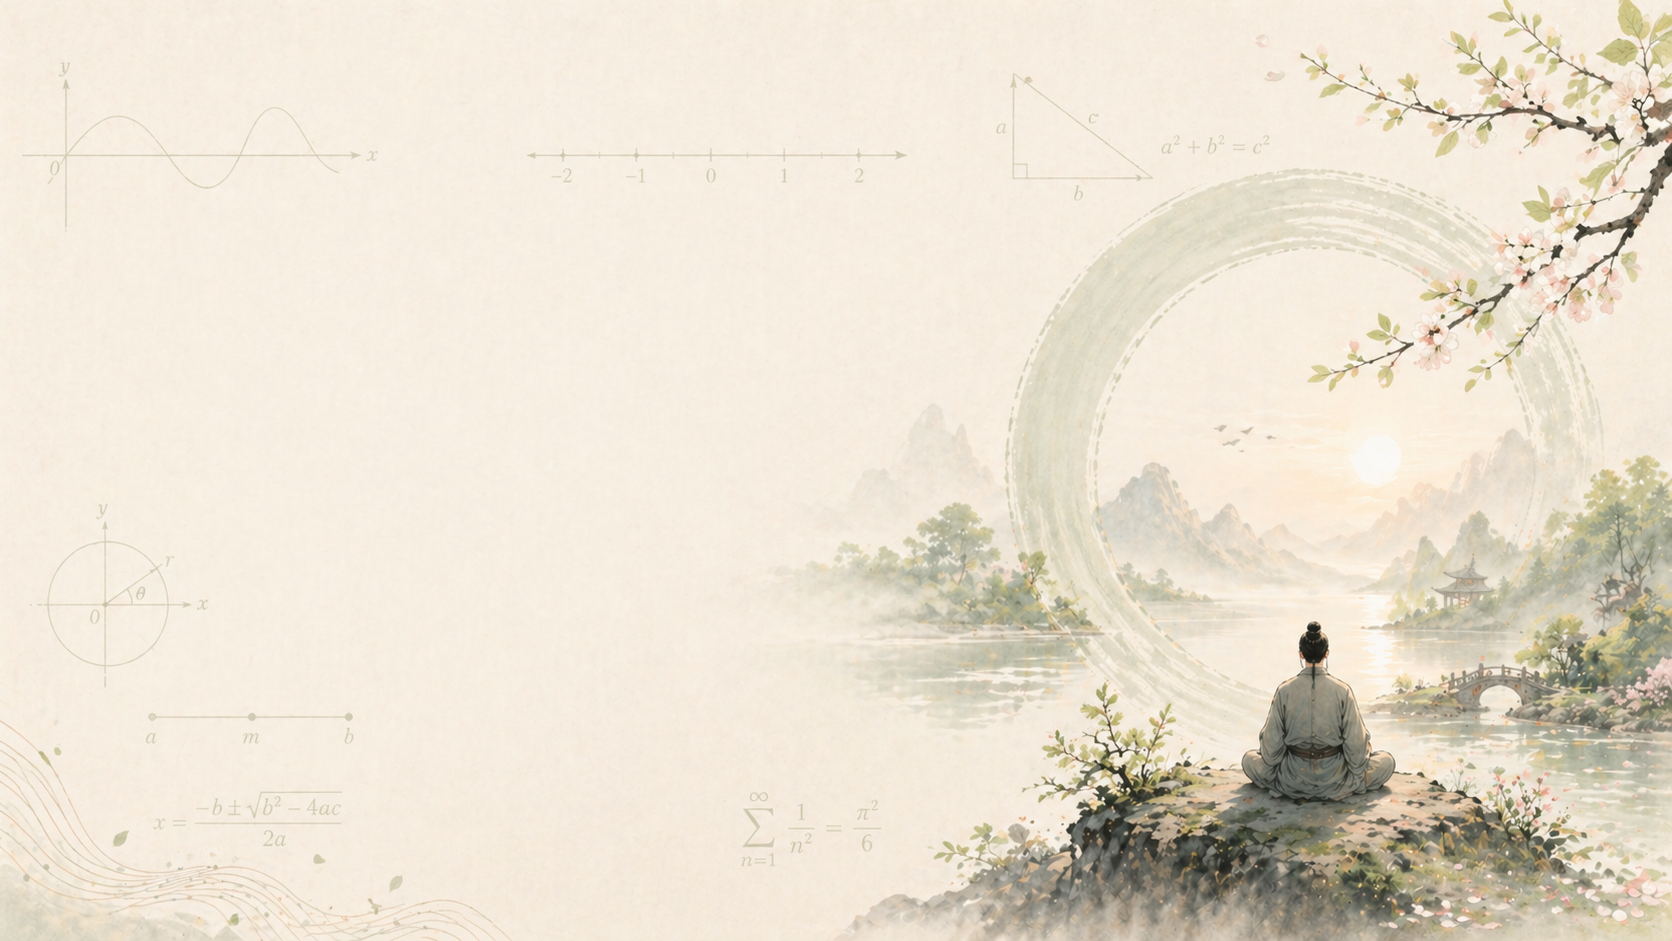
\includegraphics[width=\paperwidth,height=\paperheight,keepaspectratio=false]{chapter_03_bg_04.png}%
}
% =============================================================================
% THEOREM 3.7
% =============================================================================
\section{Subsequential Limits Form a Closed Set}

% --- Theorem 3.7 statement ---
\begin{frame}{Theorem 3.7: $E^*$ Is Closed}
  \begin{thmblock}{Theorem 3.7}
    The set $E^*$ of subsequential limits of a sequence $\{p_n\}$ in a metric space $X$ is a \alert{closed} subset of $X$.
  \end{thmblock}

  \vspace{0.4em}
  \begin{hlbox}
    \textbf{Why this matters:}
    \begin{itemize}
      \item Limits of subsequential limits are again subsequential limits.
      \item $E^*$ contains all its limit points --- nothing escapes.
    \end{itemize}
  \end{hlbox}

  \note{
    Theorem 3.7 says something quite striking. Take any sequence in any
    metric space, and look at all the points that are limits of some
    subsequence. That set, denoted "E" star, is automatically closed.
    In particular, if you have a list of subsequential limits and they
    themselves converge to some point "q", then "q" is also a
    subsequential limit. Nothing escapes the set "E" star by taking
    further limits. The proof is an inductive construction with a
    triangle-inequality squeeze, quite similar in spirit to the one
    for Theorem 3.6.
  }
\end{frame}

% --- Picture: E* as closed set ---
\begin{frame}[c]{Picture: $E^*$ as a Closed Set}
  \begin{center}
  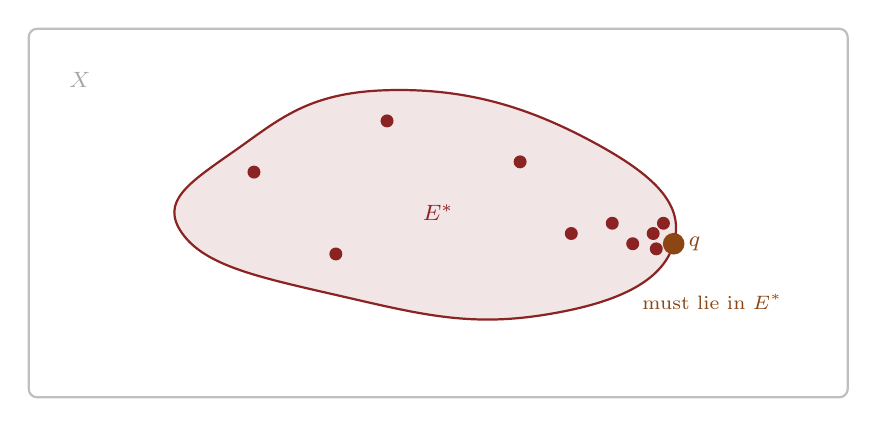
\begin{tikzpicture}[scale=1.3]
    % Ambient X
    \fill[white, opacity=0.3, rounded corners=3pt] (-4.0, -1.8) rectangle (4.0, 1.8);
    \draw[gray!50, thick, rounded corners=3pt] (-4.0, -1.8) rectangle (4.0, 1.8);
    \node[gray!70] at (-3.5, 1.3) {\footnotesize $X$};
    % E*
    \fill[thmcolor!12] plot[smooth cycle, tension=0.8] coordinates {(-2,0.6) (-0.5,1.2) (1.5,0.7) (2.3,-0.3) (1.0,-1.0) (-1,-0.8) (-2.5,-0.2)};
    \draw[thmcolor, thick] plot[smooth cycle, tension=0.8] coordinates {(-2,0.6) (-0.5,1.2) (1.5,0.7) (2.3,-0.3) (1.0,-1.0) (-1,-0.8) (-2.5,-0.2)};
    \node[thmcolor] at (0, 0.0) {\footnotesize $E^*$};
    % Points in E*
    \fill[thmcolor] (-1.8, 0.4) circle (1.8pt);
    \fill[thmcolor] (-0.5, 0.9) circle (1.8pt);
    \fill[thmcolor] (0.8, 0.5) circle (1.8pt);
    \fill[thmcolor] (-1.0, -0.4) circle (1.8pt);
    \fill[thmcolor] (1.3, -0.2) circle (1.8pt);
    \fill[thmcolor] (1.7, -0.1) circle (1.8pt);
    \fill[thmcolor] (1.9, -0.3) circle (1.8pt);
    \fill[thmcolor] (2.1, -0.2) circle (1.8pt);
    \fill[thmcolor] (2.2, -0.1) circle (1.8pt);
    \fill[thmcolor] (2.13, -0.35) circle (1.8pt);
    % q on boundary of E*
    \fill[mAccent] (2.3, -0.3) circle (3pt);
    \node[mAccent, right=2pt] at (2.3, -0.3) {\footnotesize $q$};
    % Note
    \node[mAccent, below right] at (1.9, -0.7) {\scriptsize must lie in $E^*$};
  \end{tikzpicture}
  \end{center}

  \note{
    Here is the picture. The gray box is the ambient metric space "X".
    The red shaded region is the set "E" star of subsequential limits
    of our sequence. The red dots inside are particular subsequential
    limits. Now suppose those red dots themselves converge, as a
    sequence, to some new point "q", shown in orange on the boundary.
    Theorem 3.7 says "q" is also a subsequential limit, so it must lie
    inside "E" star. The conclusion is that the boundary
    points of "E" star are themselves in "E" star, which is exactly
    what closed means.
  }
\end{frame}

% --- Proof of 3.7 strategy ---
\begin{frame}{Proof Strategy: Theorem 3.7}
  \begin{hlbox}
    \textbf{Goal:} Show every limit point $q$ of $E^*$ lies in $E^*$.

    \vspace{0.5em}
    \textbf{Approach:} Build a subsequence $\{p_{n_k}\}$ of $\{p_n\}$ with $p_{n_k} \to q$.

    \vspace{0.5em}
    \textbf{Trick:} Use \alert{both} facts at each step:
    \begin{itemize}
      \item ``$q$ is a limit point of $E^*$'' $\Longrightarrow$ pick $x \in E^*$ near $q$.
      \item ``$x \in E^*$'' $\Longrightarrow$ pick $p_{n_k}$ near $x$.
    \end{itemize}
    Triangle inequality then forces $p_{n_k}$ near $q$.
  \end{hlbox}

  \note{
    Here is the high-level idea. To prove "E" star is closed we take
    any limit point "q" of "E" star and show "q" itself lies in "E"
    star. To do that, we have to exhibit a subsequence of the original
    sequence "p" sub "n" that converges to "q". The trick is to use
    the two facts available at each step. First, "q" is a limit point
    of "E" star, so we can find a subsequential limit "x" close to "q".
    Second, "x" is a subsequential limit, so we can find an actual term
    of the original sequence close to "x". Combining via the triangle
    inequality, the term we picked is close to "q". By tightening the
    closeness to one over "k" at step "k", the bound shrinks like two
    over "k" and we get convergence.
  }
\end{frame}

% --- Proof 3.7 Step 1 ---
\begin{frame}{Proof of 3.7 --- Step 1: Setup}
  \begin{proofblock}{Step 1 --- the construction plan}
    Let $q$ be a limit point of $E^*$.

    \vspace{0.3em}
    Set $n_0 = 0$ (so that ``$n_k > n_{k-1}$'' makes sense at $k = 1$).

    \vspace{0.3em}
    We will build $0 < n_1 < n_2 < n_3 < \cdots$ inductively so that
    \[
      d(q, p_{n_k}) \to 0 \quad \text{as } k \to \infty .
    \]
  \end{proofblock}

  \note{
    Step 1: setup. Let "q" be a limit point of "E" star. Our goal is
    to produce a subsequence of the original sequence that converges
    to "q". Note that the assumption already gives us enough room to
    work with: a single-point set has no limit points, so "q" being a
    limit point of "E" star forces "E" star to contain other points
    besides "q". We adopt the convention that "n" sub 0 equals zero,
    purely as a starting peg so that the constraint "n" sub "k"
    greater than "n" sub "k" minus one makes sense even when "k"
    equals one. Then we pick the indices "n" sub 1, "n" sub 2, "n"
    sub 3, and so on inductively, ensuring that the distance from
    "q" to the "k"-th chosen term shrinks toward zero as "k" grows.
  }
\end{frame}

% --- Proof 3.7 Step 2 ---
\begin{frame}{Proof of 3.7 --- Step 2: Inductive Choice}
  \begin{proofblock}{Step 2 --- inductive choice of $n_k$}
    Suppose $n_1, \dots, n_{k-1}$ are chosen. Pick:
    \begin{itemize}
      \item $x \in E^*$ with $d(x, q) < \dfrac{1}{k}$ \;\;(possible: $q$ is a limit point of $E^*$).
      \item $n_k > n_{k-1}$ with $d(x, p_{n_k}) < \dfrac{1}{k}$ \;\;(possible: $x \in E^*$).
    \end{itemize}
  \end{proofblock}

  \note{
    Step 2: the inductive step. Assume the first "k" minus one indices
    have already been chosen. Now we pick the next one in two
    sub-stages. First, because "q" is a limit point of "E" star, the
    open ball of radius one over "k" around "q" contains some point
    "x" of "E" star, in fact infinitely many. Pick any such "x".
    Second, because "x" itself is a subsequential limit, some
    subsequence of the original sequence converges to "x". So
    infinitely many original terms lie within distance one over "k" of
    "x". In particular, we can find such a term with index strictly
    greater than "n" sub "k" minus one. Call its index "n" sub "k".
  }
\end{frame}

% --- Proof 3.7 Step 3 ---
\begin{frame}{Proof of 3.7 --- Step 3: Triangle Inequality}
  \begin{proofblock}{Step 3 --- estimate $d(q, p_{n_k})$}
    By the triangle inequality:
    \[
      d(q, p_{n_k}) \leq d(q, x) + d(x, p_{n_k}) < \frac{1}{k} + \frac{1}{k} = \frac{2}{k} .
    \]
    Hence
    \[
      \boxed{\, d(q, p_{n_k}) < \frac{2}{k} \quad \text{for all } k \geq 1. \,}
    \]
  \end{proofblock}

  \note{
    Step 3: combine the two estimates. The distance from "q" to the
    chosen term "p" sub "n" sub "k" is at most the distance from "q"
    to "x" plus the distance from "x" to that term, by the triangle
    inequality. Each summand is less than one over "k" by
    construction, so the total is less than two over "k". The boxed
    conclusion records the uniform bound: for every "k", the distance
    from "q" to the "k"-th subsequential term is less than two over
    "k".
  }
\end{frame}

% --- Proof 3.7 Step 4 ---
\begin{frame}{Proof of 3.7 --- Step 4: Conclusion}
  \begin{proofblock}{Step 4 --- $\{p_{n_k}\}$ converges to $q$}
    Since $2/k \to 0$ as $k \to \infty$:
    \[
      d(q, p_{n_k}) \to 0 \quad \Longrightarrow \quad p_{n_k} \to q.
    \]
    So $q \in E^*$.

    \vspace{0.3em}
    Hence $E^*$ contains all its limit points: $E^*$ is \alert{closed}. \quad $\Box$
  \end{proofblock}

  \note{
    Step 4 finishes the argument. The bound two over "k" tends to zero
    as "k" tends to infinity. So the distance from "q" to "p" sub "n"
    sub "k" tends to zero, which is exactly what it means for the
    subsequence to converge to "q". Hence "q" is itself a subsequential
    limit of the original sequence, so "q" lies in "E" star. Since "q"
    was an arbitrary limit point of "E" star, the set "E" star contains
    all of its limit points, which is the definition of being closed.
    The proof is complete.
  }
\end{frame}
}

{
\usebackgroundtemplate{%
  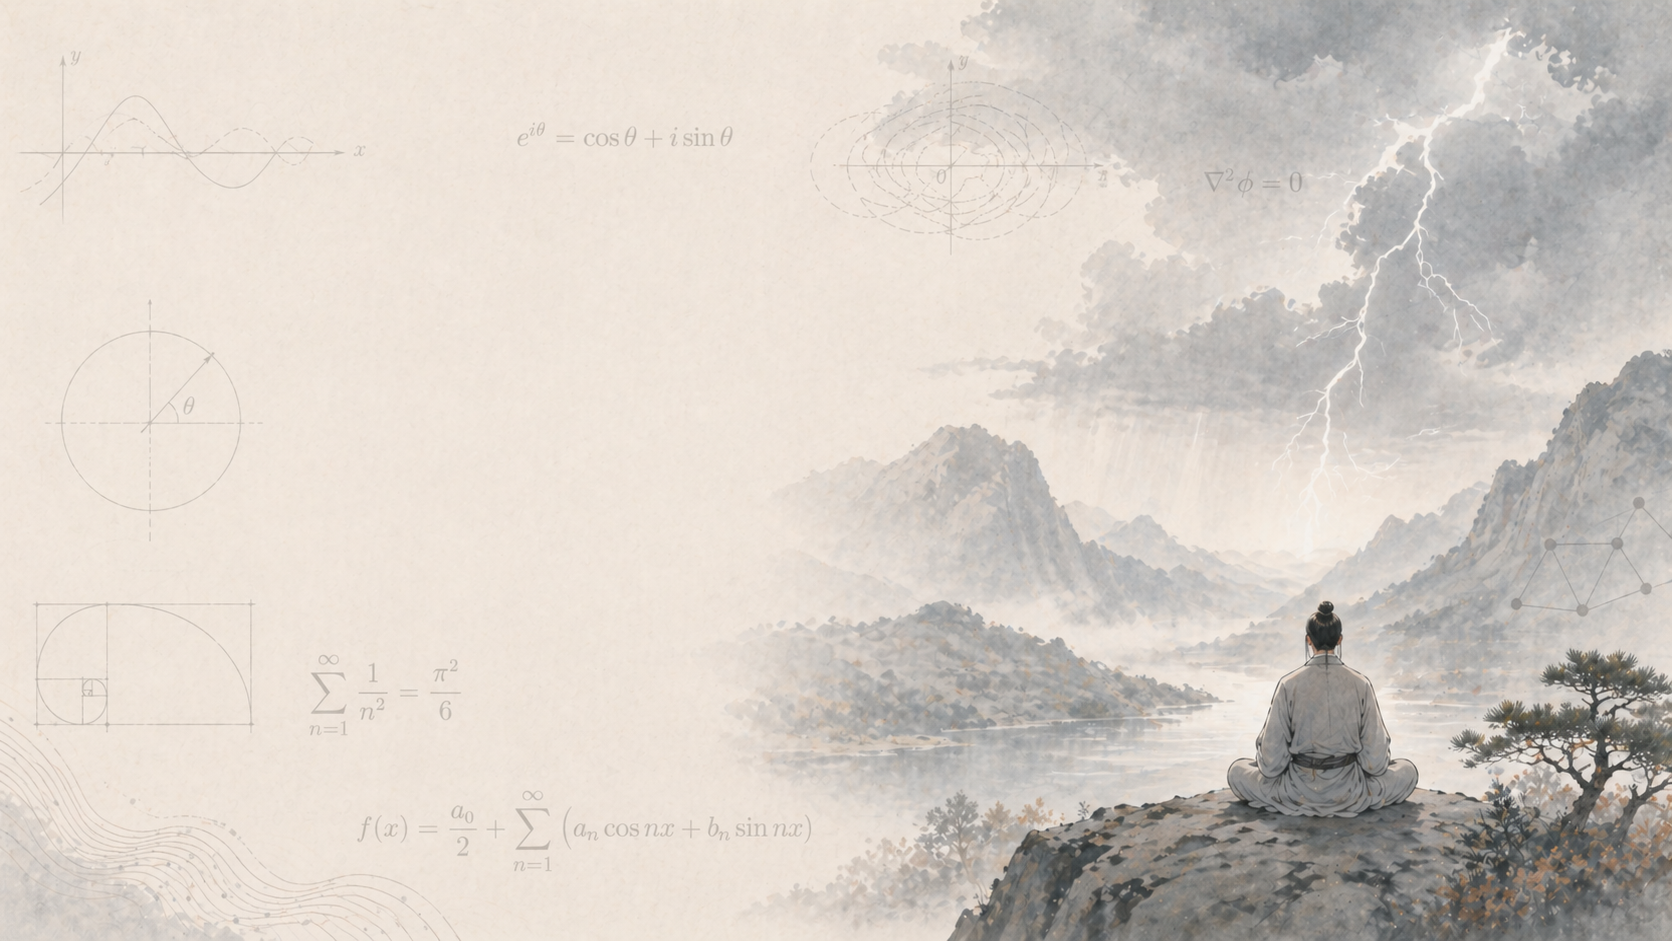
\includegraphics[width=\paperwidth,height=\paperheight,keepaspectratio=false]{chapter_03_bg_05.png}%
}
% =============================================================================
% SUMMARY
% =============================================================================
\section{Summary}

% --- Summary build 1/4 ---
\begin{frame}{Summary}
  \begin{hlbox}
    \textbf{Key takeaways:}
    \begin{itemize}
      \item \alert{Definition 3.5:} subsequence $\{p_{n_k}\}$ via strictly increasing indices.
    \end{itemize}
  \end{hlbox}

  \note{
    Let us recap. First, Definition 3.5: a subsequence is what you get
    by reading off an original sequence at a strictly increasing
    sequence of indices. The order of terms is preserved, and we keep
    infinitely many of them. Limits of convergent subsequences are
    called subsequential limits, and the set of all such limits is
    denoted "E" star.
  }
\end{frame}

% --- Summary build 2/4 ---
\begin{frame}{Summary}
  \begin{hlbox}
    \textbf{Key takeaways:}
    \begin{itemize}
      \item \alert{Definition 3.5:} subsequence $\{p_{n_k}\}$ via strictly increasing indices.
      \item \alert{Convergence test:} $p_n \to p$ iff every subsequence converges to $p$.
    \end{itemize}
  \end{hlbox}

  \note{
    Second, the convergence test. A sequence converges to "p" if and
    only if every one of its subsequences also converges to "p". This
    gives a useful way to disprove convergence, by exhibiting two
    subsequences with different limits, as we did with the alternating
    plus-minus-one example.
  }
\end{frame}

% --- Summary build 3/4 ---
\begin{frame}{Summary}
  \begin{hlbox}
    \textbf{Key takeaways:}
    \begin{itemize}
      \item \alert{Definition 3.5:} subsequence $\{p_{n_k}\}$ via strictly increasing indices.
      \item \alert{Convergence test:} $p_n \to p$ iff every subsequence converges to $p$.
      \item \alert{Theorem 3.6:} compact $\Rightarrow$ a convergent subsequence exists; bounded in $\mathbb{R}^k \Rightarrow$ same.
    \end{itemize}
  \end{hlbox}

  \note{
    Third, Theorem 3.6, the existence theorem. In any compact metric
    space, every sequence has a subsequence that converges to a point
    of the space. Specialised to euclidean space, every bounded
    sequence in "R" to the "k" has a convergent subsequence. This is
    the Bolzano-Weierstrass theorem, and it is one of the workhorses
    of the rest of the book.
  }
\end{frame}

% --- Summary build 4/4 ---
\begin{frame}{Summary}
  \begin{hlbox}
    \textbf{Key takeaways:}
    \begin{itemize}
      \item \alert{Definition 3.5:} subsequence $\{p_{n_k}\}$ via strictly increasing indices.
      \item \alert{Convergence test:} $p_n \to p$ iff every subsequence converges to $p$.
      \item \alert{Theorem 3.6:} compact $\Rightarrow$ a convergent subsequence exists; bounded in $\mathbb{R}^k \Rightarrow$ same.
      \item \alert{Theorem 3.7:} the set $E^*$ of subsequential limits is closed.
    \end{itemize}

    \vspace{0.5em}
    \textbf{Coming up next:} Cauchy sequences.
  \end{hlbox}

  \note{
    Fourth, Theorem 3.7. The set "E" star of all subsequential limits is
    a closed subset of the metric space, no matter how the original
    sequence behaves. The proof was a clever two-step approximation:
    pick a subsequential limit close to "q", then pick an actual term
    close to that limit, and use the triangle inequality. Coming up
    next we turn to Cauchy sequences. There we will see a different
    way to certify convergence, one that does not require us to guess
    the limit in advance.
  }
\end{frame}
}

\end{document}
